\section{comparison}
\subsection{t<0}

\begin{table}[h]
\begin{center}
  \begin{tabular}{|c|c|}
    \hline    
    {\bf Name} & {\bf Value [mA or V]} \\ \hline
    $I_b$ & -2.658976e-04
$I_c$ & 0
$I_R$$_1$ & 2.536488e-04
$I_R$$_2$ & 2.658976e-04
$I_R$$_3$ & -1.224882e-05
$I_R$$_4$ & 1.205310e-03
$I_R$$_5$ & -2.658976e-04
$I_R$$_6$ & 9.516615e-04
$I_R$$_7$ & 9.516615e-04
$V_1$ & 5.054819
$V_2$ & 4.793705
$V_3$ & 4.258198
$V_4$ & 4.831047
$V_5$ & 5.668298
$V_6$ & -1.934226
$V_7$ & -2.905231
$V_8$ & -1.934226

    \hline
  \end{tabular}
  \begin{tabular}{|c||c|}
    \hline    
    {\bf Name} & {\bf Value [A or V]} \\ \hline
    \input{../sim/op1_tab}
    \hline
  \end{tabular}
  \caption{Comparison 1}
  \label{tab:comparison 1}
\end{center}
\end{table}
\FloatBarrier

\subsection{Equivalent resistance}
%Para esta acho que nao vale a pena estar a imprimir as tabelas. Basta referir os valores do Req.
%\begin{table}[h]
%\begin{center}
 % \begin{tabular}{|c|c|}
  %  \hline    
   % {\bf Name} & {\bf Value [mA or V]} \\ \hline
    %$I_b$ & 0.000000
$I_R$$_1$ & 0.000000
$I_R$$_2$ & 0.000000
$I_R$$_3$ & 0.000000
$I_R$$_4$ & 0.000000
$I_R$$_5$ & -2.722816e-03
$I_R$$_6$ & -0.000000
$I_R$$_7$ & 0.000000
$V_1$ & 0.000000
$V_2$ & 0.000000
$V_3$ & 0.000000
$V_4$ & 0.000000
$V_5$ & 8.573530
$V_6$ & 0.000000
$V_7$ & 0.000000
$V_8$ & 0.000000
$V_X$ & 8.573530
$I_X$ & -2.722816e-03
$R_e$$_q$ & -3148.773562
$tau$ & -3.239206e-03
$I_b$ & 0.000000
$I_R$$_1$ & 0.000000
$I_R$$_2$ & 0.000000
$I_R$$_3$ & 0.000000
$I_R$$_4$ & 0.000000
$I_R$$_5$ & -2.722816e-03
$I_R$$_6$ & -0.000000
$I_R$$_7$ & 0.000000
$V_1$ & 0.000000
$V_2$ & 0.000000
$V_3$ & 0.000000
$V_4$ & 0.000000
$V_5$ & 8.573530
$V_6$ & 0.000000
$V_7$ & 0.000000
$V_8$ & 0.000000
$V_X$ & 8.573530
$I_X$ & -2.722816e-03
$R_e$$_q$ & -3148.773562
$tau$ & -3.239206e-03
$I_b$ & 0.000000
$I_R$$_1$ & 0.000000
$I_R$$_2$ & 0.000000
$I_R$$_3$ & 0.000000
$I_R$$_4$ & 0.000000
$I_R$$_5$ & -2.722816e-03
$I_R$$_6$ & -0.000000
$I_R$$_7$ & 0.000000
$V_1$ & 0.000000
$V_2$ & 0.000000
$V_3$ & 0.000000
$V_4$ & 0.000000
$V_5$ & 8.573530
$V_6$ & 0.000000
$V_7$ & 0.000000
$V_8$ & 0.000000
$V_X$ & 8.573530
$I_X$ & -2.722816e-03
$R_e$$_q$ & -3148.773562
$tau$ & -3.239206e-03

   % \hline
  %\end{tabular}
  %\begin{tabular}{|c||c|}
   % \hline    
   % {\bf Name} & {\bf Value [A or V]} \\ \hline
   % \input{../sim/op2_tab}
   % \hline
  %\end{tabular}
  %\caption{Comparison 2}
 % \label{tab:comparison 2}
%\end{center}
%\end{table}
%\FloatBarrier

\subsection{Natural solutin $V_5$}


\begin{figure}[h] \centering
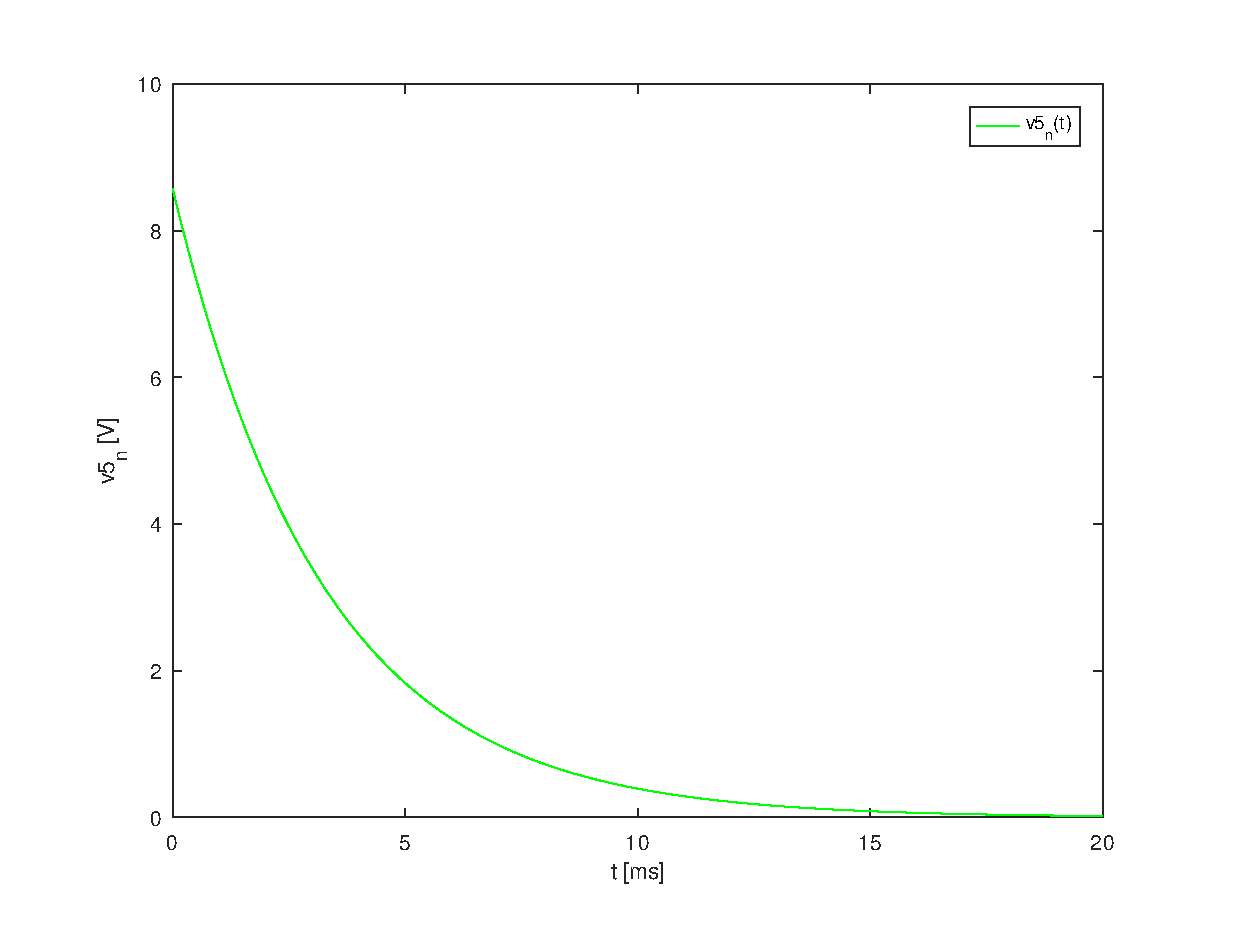
\includegraphics[scale=0.4]{v5_n.eps}
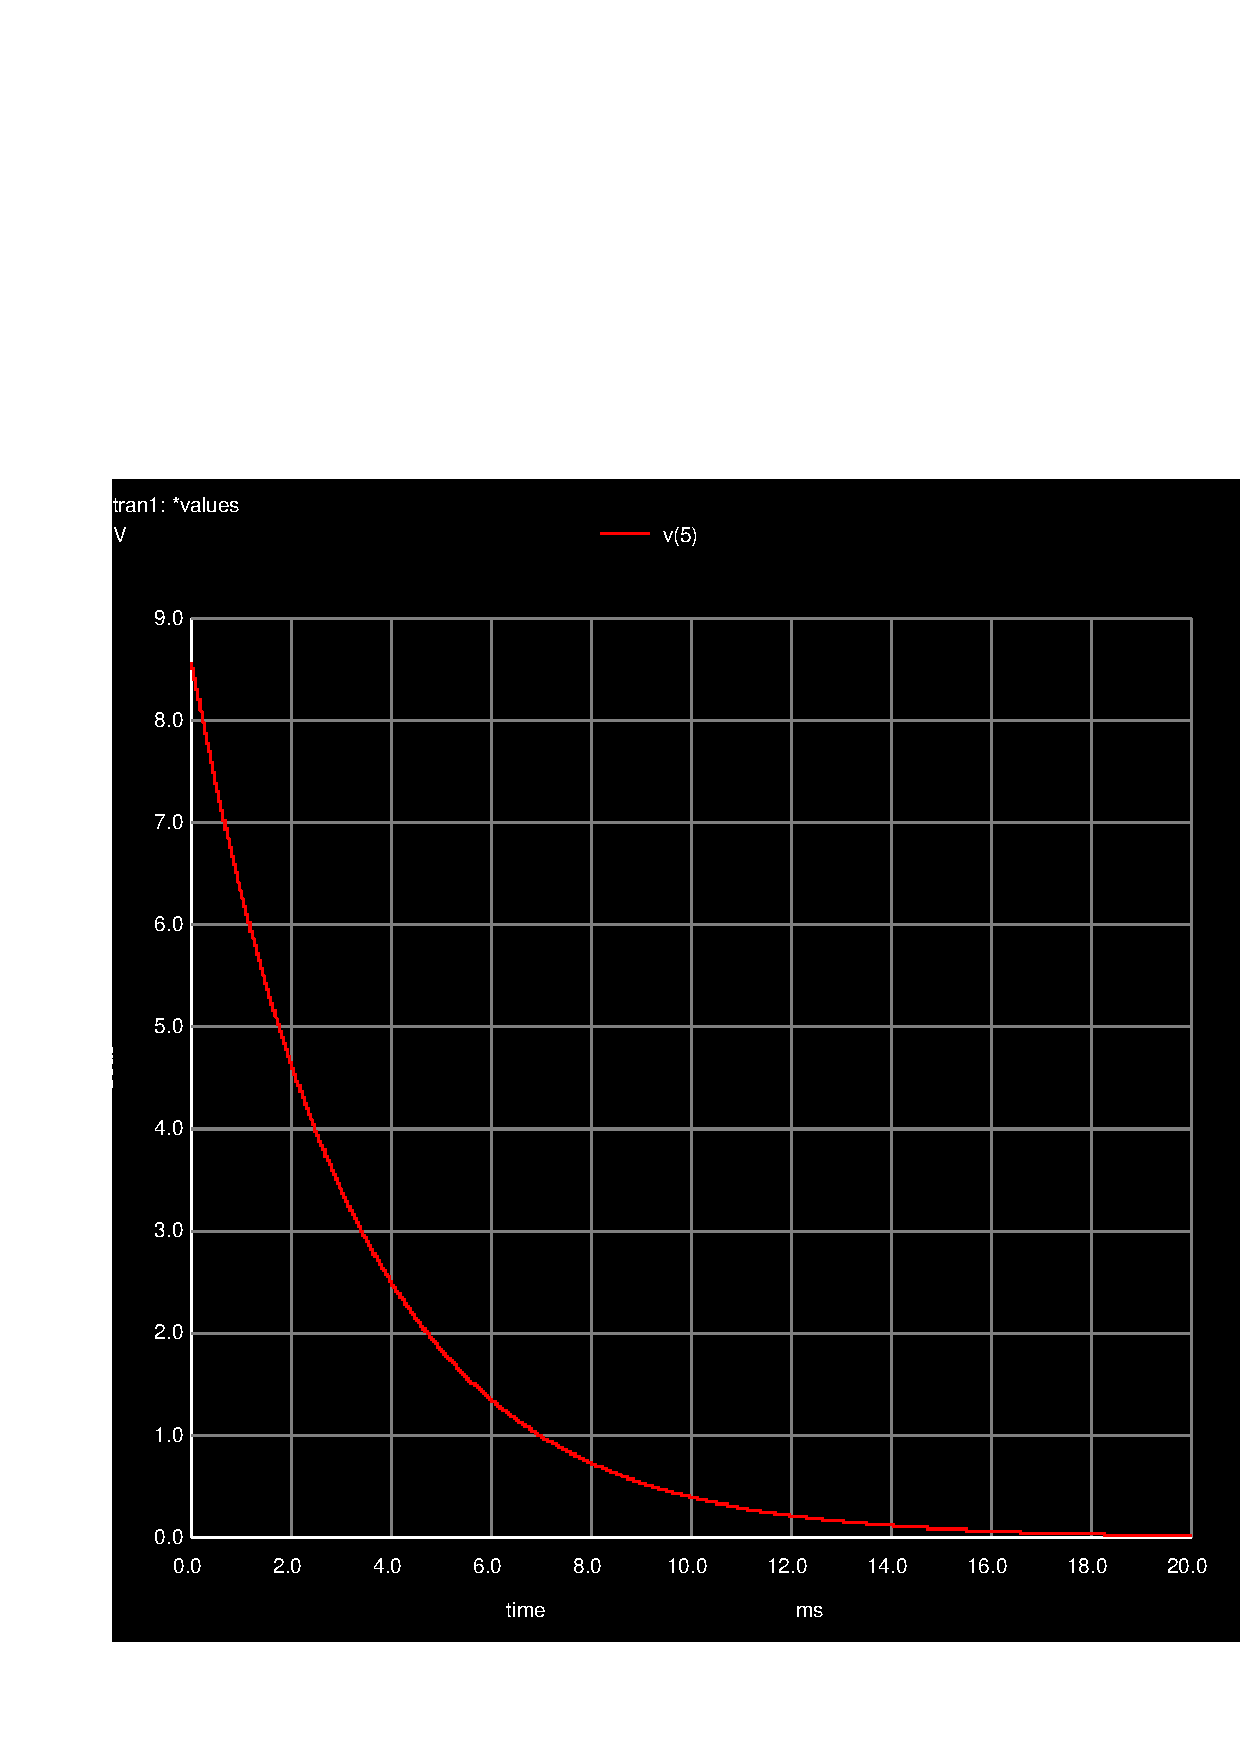
\includegraphics[scale=0.3]{transv5n.pdf}
\caption{Natural solution V5}
\label{fig:comparison5}
\end{figure}
\FloatBarrier


\section{Conclusion}
\label{sec:conclusion}
Comparing the results given by Nodal and Mesh analysis, it can be observed that both methods achieved the same values. Also, the results given by the Ngspice simulation are the same as those of the methods stated above.  
All in all, the analysis of the given circuit using the stated methods was achieved successfully. Nodal and mesh methods were performed both theoretically using the Octave maths tool and by circuit simulation using the Ngspice software. 
Given the fact that the circuit only has linear components and it is a simple circuit to analyse, Ngspice probably used the same models as we did in the theoretical analysis, so it makes sense that no discrepancies were detected. However, if we had been given a circuit with more complex components, the theoretical and simulation models could not match as precisely as they did in this laboratory assignment. 

